\subsection{Comment indexer les données automatiquement produites ? : interface d’indexation} - Processus côté interface 

L’objet de notre étude est le reversement des données produites par l’indexation automatique au sein du modèle FRBR, adapté aux archives audiovisuelles. Si les outils d’extraction automatique tels que YOLOv8, nécessitent un réentrainement spécifique au corpus étudié, une seconde difficulté s'impose, celle de l'alignement de ces données avec un modèle de données personnalisé. Le modèle de données FRBR est, en effet, configuré selon les besoins métier de chaque institution et conditionne l’organisation des données pour l’utilisateur au sein de l’interface. Dès lors, comment reverser des données produites automatiquement, au sein d’un modèle de données configurable ? Ce reversement concrétise en effet l’indexation automatique, puisque les données deviennent visibles et requêtables par les utilisateurs, au sein de l'interface du logiciel. 

%Faire le lien avec le NLP le plus possible : le NLP pourra être étendu pour la recherche de contenus visuels  

%Yolo est une IA discriminative 

\subsubsection{Reversement des données au sein du FRBR} 

FRBRisation des données générées par IA  


Une fois les deux processus de segmentation et de détection d'objets finalisés, deux types de données sont produits : les time codes, chiffrés, et les mots-clés, textuels et sémantiques. L'enjeu est de structurer ces données au sein du modèle FRBR existant. 

%Certains outils ont déjà été développés dans d’autres applications de gestion des collections afin d’effectuer ce reversement de manière automatique : Wedia, Keepeek, Einden, MomaSoft “classent automatiquement les images et vidéos en leur attribuant les métadonnées appropriées.” \footcite{zotero-item-732}

Création d'une nouvelle entité : 
Les outils automatiques utilisés lors du processus ont extrait des données depuis un média, associé au niveau de l'item numérique au sein du modèle de données préexistant. Or, le niveau item contient des éléments de description matérielle techniques, alors que les mots-clés et repères temporels relèvent d'une description intelectuelle et syntaxique. Dès lors, la création d'une entité intelectuelle dédiée à la séquence s'impose. 
Afin d'illustrer l'intégration d'une entité de description intermédiaire, entre l'oeuvre et l'item numérique, prenons l'exemple de la plateforme Okapi (Open and Knowledge-based Annotation and Publishing Interface), développée par le département Recherche et Innovation de l'\gls{ina} \footcite{lalande2022}. Afin de favoriser la description collaborative de contenus multimédias, la plateforme offre la possibilité aux utilisateurs de concevoir des modèles de description personnalisés \footcite{lalande2022}. La plateforme permet notamment de séparer l'extrait audiovisuel du média, dont il constitue un niveau descriptif propre. Une strate supplémentaire de description est ainsi dédiée à la description intellectuelle du média. Le modèle FRBR tel que nous l'avons décrit ne propose, a priori, pas d'entité descriptive dédiée à la séquence. L'entité "d'agrégats", proposée par le manuel de la \gls{fiaf} pourrait y correspondre. Toutefois, ceux-ci “sont conçus et créés dès le début pour rassembler plusieurs composantes individuelles formant un tout." \footcite{zotero-item-646}. Or, au sein du corpus étudié, les rushes ne font pas partie d'un montage. Toute segmentation est une interprétation a posteriori de la construction de l’archive, et donc un remontage. L'entité de "fragment d'expression" proposé par l'IFLA au sein du modèle FRBR bibliographique semble plus adéquate \footcite{iflastandards.info2026}. L’\gls{IFLA} définit le fragment comme “des parties d’expressions qui ne constituent pas elles-mêmes des expressions autonomes.[...] Un « Fragment d’expression » n’est identifié qu’en fonction de son occurrence au sein d’un tout connu ou supposé.” \footcite{iflastandards.info2026}. Cette entité semble correspondre à la notion de séquences telle que nous l'avons décrite. Elle serait rattachée à l’Oeuvre, conformément à l’adaptation du FRBR par les recommandations de la FIAF, et permettrait le reversement spécifique des times-codes et mots-clés. La figure \ref{figfragment} ci-dessous illustre l'intégration de l'entité du fragment d'oeuvre au modèle de données existant. 

\begin{figure}[htbp] 
	
	\centering 
	
	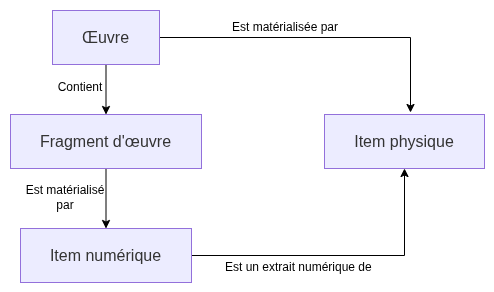
\includegraphics[width=0.7\textwidth]{images/fragment_frbr.png} 
	
	\caption{Intégration du Fragment au modèle de données} 
	
	\label{figfragment} 
	
\end{figure} 

Au sein de la plateforme Okapi, la création d'une entité intermédiaire de description, permet aux données descriptives produites à partir du média, d'être reversées au sein d'un niveau parent essentiellement descriptif, celui de l'extrait. Au sein du modèle de données existant, adapté au corpus étudié, les time codes et les mots-clés sont déjà indexés manuellement en tant que données au sein de l’application. En effet, les times codes sont renseignés au niveau de l'item numérique, dans un champ notes, et l'item comporte le champ type renseigné par la valeur “fichier time codé”, afin de signifier sa qualité d'extrait. De plus, les mots-clés sont renseignés au niveau de l’indexation de l’œuvre, donc du rush original. La modélisation de la segmentation au sein du modèle actuel implique un nombre conséquent de relations entre les éléments, complexifiant ainsi la navigation de l'utilisateur. En effet, une notice d'item physique renseigne tous les extraits numériques (items numériques) qui lui sont liés. L’item numérique (segment) renseigne le film physique duquel il est extrait, tandis que le niveau œuvre renseigne uniquement les extraits numériques qui lui sont associés. 
La création d’une nouvelle entité simplifierait la navigation au sein de l'interface et permettrait de séparer la description en différents niveaux, intellectuel et technique, conformément aux principes du FRBR. La nouvelle entité de fragments permettrait éventuellement de préciser un contexte de segmentation et des champs dédiés aux mots clés et aux time codes. Le tableau \ref{tab:reversement_metadonnees_frbr} ci-dessous illustre la répartition de la description entre le fragment d'Oeuvre et l'item numérique. Pour des raisons de clarté, d'autres données descriptives ont été intégrées afin d'illustrer la répartition entre la description intellectuelle et matérielle. 

\begin{table}[H]
	\centering
	\small
	\renewcommand{\arraystretch}{1.3}
	\begin{tabular}{|p{3.8cm}|p{4.2cm}|p{6.4cm}|}
		\hline
		\textbf{Entité FRBR} & \textbf{Champ / Attribut} & \textbf{Exemples de valeurs} \\
		\hline
		\multirow{6}{=}{\textbf{Fragment d’Oeuvre} \newline \textit{(Description intellectuelle)}} 
		& Contexte & Segmentation automatique de tel item physique \\ \cline{2-3}
		& Description générale & Description du contenu sémantique de la séquence \\ \cline{2-3}
		& Processus de segmentation & Automatique (Outil utilisé et paramètres appliqués) \\ \cline{2-3}
		& Time codes & Time codes de début et de fin de la séquence \\ \cline{2-3}
		& Mots-clés & Mots-clés extraits par YOLO \\ \cline{2-3}
		& Image-clé associée & Lien direct vers le fichier de l'image-clé \\ \cline{2-3}
		& Oeuvre parente & Identifiant de l'oeuvre associée, lien direct vers la notice \\ \cline{2-3}
		& Item physique associé & Identifiant de l'item physique associé dont est tirée la séquence, lien direct vers la notice \\ \cline{2-3}
		& Item numérique associé & Identifiant de l'item numérique associé, lien direct vers la notice \\ 
		\hline
		\multirow{3}{=}{\textbf{Item Numérique} \newline \textit{(Description technique et matérielle)}} 
		& Fragment associé & Identifiant du fragment associé, lien direct vers la notice \\ \cline{2-3}
		& Données techniques & Résolution de l'image, taille, format \\ \cline{2-3}
		& Données de conservation & Emplacement, contenant \\ \cline{2-3}
		& Média associé & fichier média de la séquence \\ \cline{2-3}
		\hline
	\end{tabular}
	\caption{Attributs et exemples de valeurs associées aux entités Fragment d'Expression et Item Numérique.}
	\label{tab:reversement_metadonnees_frbr}
\end{table}

Les métadonnées automatiquement produites seraient intégrées au niveau du fragment, tandis que l'item numérique contiendrait le média et les données techniques. 
Une difficulté subsiste toutefois. En effet, les processus s'exécutent au niveau du fichier numérique et de son média, tandis que les métadonnées produites doivent pouvoir enrichir un niveau descriptif supérieur, celui du fragment. Dexu configurations peuvent être envisagées afin d'opérer ce reversement automatiquement. D'une part, l'application gère actuellement l'héritage des données d'un niveau supérieur à un niveau inférieur via la configuration de méta-masques, qui ciblent les niveaux iférieurs au sein desquels reverser les données. Néanmoins, le processus automatisé décrit impliquerait la configuration de masques ascendants, permettant de reverser des métadonnées générées au niveau de l'item, vers l'entité de fragment. Cette configuration complexifie toutefois la compréhension du modèle de données.
D'autre part, pourrait être envisagé la mise en place d'un tableau de correspondance ou d'un script permettant d'associer les sorties de données du processus aux entités dans lesquelles elles doivent être injectées. 

%À l’ingest : données interdépendantes entre la description d’un item numérique et de son média. Mentionner la relation nouvelle sur l’item numérique et son média : facilite les choses pour le reversement  
 %Pour les times codes, des champs dédiés devrons être prévus sous le champ film associé.  
%Faire un schéma de métadonnées pour pouvoir adapter les données aux normes du logiciel via des connecteurs par exemple.  

\subsubsection{Interface de validation pour l'utilisateur} 

Deux axes : visualisation et validation (intégrer à ces deux axes la transparence sur le processus : données de gestion)  

Processus d’interface avec ce nouveau schéma de données  

(Proposer un diagramme de décision pour exposer le processus interface utilisateur)  

Le changement au niveau du modèle FRBR s’effectue en backend de l’application, par les équipes techniques et els équipes métiers afin de préparer l’application à l’implémentation de processus automatiques. Toutefois, comment le processus automatique de segmentation puis d’indexation est-il représenté au sein de l’interface, pour l’utilisateur ?  

D’abord théorie, puis mise en application dans l’exemple de l’application. D'abord lire ce que j’ai écrit en citations.  

Nous pouvons imaginer le processus suivant en frontend, dans l’interface visible de l’application pour l’utilisateur. L’utilisateur procède à l’ingest d’un fichier numérisé d’une œuvre/rushe dans sa globalité. L’ingest d’un fichier numérique vidéo devrait pouvoir déclencher la proposition suivante pour l’utilisateur : Souhaitez-vous segmenter automatiquement ce fichier ? Une infobulle devrait indiquer à l’utilisateur ce qu’implique cette segmentation automatique, le processus expliqué en quelques phrases. En effet, au début de l’implémentation du processus et pour tout nouvel utilisateur confronté à cette nouvelle fonctionnalités automatiques, il est recommandé d’être “familiarisé” au “fonctionnement et limites” de ces outils, comme par exemple “la manière dont sont produites les sorties, les éventuels transferts de données, ainsi que les usages autorisés et les usages interdits."\footcite{zotero-item-729} Ces informations pourront notamment aider l’utilisateur à pouvoir valider, par la suite, les données produites par les pipelines automatisés. Skinsoft prévoit par exemple déjà des modes d’emploi à l’attention des utilisateurs lors de la livraison de nouvelles fonctionnalités. Toutefois, les informations relatives au processus devront être intégrées à l’interface et au processus, pour des soucis de transparence et de création conforme des données. Ainsi, "l’intégration de briques d’IA générative dans un système d’information (SI) devrait être pensée avec des éléments de design informant clairement les utilisateurs de l’origine de la proposition, leur rappelant qu’il leur revient de ne pas prendre « telle quelle » la proposition. Par exemple, le système peut proposer pour chaque question au moins deux réponses, ce qui permet à l’opérateur humain de sélectionner les éléments pertinents de chaque réponse pour consolider la sienne." \footcite{zotero-item-729} Au lieu de proposer deux réponses, ce qui surchargerait l’interface, et de plus, ce n’est pas adapté ici puisque le processus de segmentation n’utilise pas d’intelligence artificielle capable de raisonner. Nous pourrions proposer, si l’utilisateur ne valide pas les données produites, la possibilité de "permettre CROCHETS un point de contact pour remonter des problèmes ou des difficultés d’ordre éthique"\footcite{zotero-item-729}. L’interface devra ainsi prévoir un formulaire décrivant la raison du refus des données, envoyé à l’équipe technique afin que le processus puisse être amélioré au niveau de ses paramètres. Ainsi, dan sles premiers mois de sa mise en place, l’implémentation pourra faire l’objet d’essais erreurs auprès des utilisateurs afin de pouvoir être perfectionné. Selon les recommandations du livre blanc : "lors des premiers mois et années de l’utilisation des IA, il est recommandé de recueillir régulièrement l’avis des utilisateurs finaux sur l’utilité et les limites du système"\footcite{zotero-item-729} 

En effet, il faudra également lui indiquer les actions qu’il va devoir effectuer au cours du processus. En effet, il devra être demandé à l’utilisateur de valider ou non, les données produites.  

La validation est utile à la responsabilisation des utilisateurs pour l’usage des outils d’automatisation en les “incitant à vérifier les données fournies en entrée et la qualité des sorties " \footcite{zotero-item-729} Les outils d’automatisation doivent être des facilitateurs sans rendre l’indexation trop automatique et facile. L’interface doit prévoir ces étapes de validation de manière simple pour l’utilisateur. \footcite{zotero-item-632}

Les données de gestion sur la production de ces données doivent être automatiquement enregistrées par l’application : quel est l’outil utilisé, le processus effectué, qui a validé, quand... L’application prévoit déjà un enregistrement des données de gestion et de l’historique des modifications automatique sur les notices via un menu spécifique. Un nouveau menu pourrait être créé pour les données de gestion automatiques des notices.  

Une fois que le fichier numérique a été segmenté, l’interface doit pouvoir présenter à l’utilisateur les times codes choisis avec l’image clé associée pour que l’utilisateur puisse visualiser les coupures qui ont été sélectionnées en accord avec les différences entre les images. Si l’utilisateur valide la segmentation, l’interface indexe les time codes sur le fichier numérique associé automatiquement dans le champ dédié, propose la génération de mots clés sur les segments générés : l’utilisateur pourra alors choisir s’il veut appliquer la génération de mots clés sur tous les segments ou seulement des segments spécifiques sous la forme d’une sélection.  
Une fois le processus de génération de mots clés terminé, l’interface propose à l’utilisateur de valider les mots clés en accord avec les images clés analysées.  

Si l’utilisateur ne valide pas les segments, ou n’en valide qu’une partie : il sera important d’intégrer à l’interface un formulaire d’erreurs qui explique les raisons du refus, afin de perfectionner l’algorithme de détection de segmentations. Même chose pour les mots clés. Pour les mots clés, l’interface peut proposer à l’utilisateur de modifier manuellement les mots clés pour les indexer mais aussi m-pour les renvoyer au modèle et alimenter le jeu de données sur lequel il s’entraîne.  

À l’INA, les chercheurs ont développé Amalia.Js, un lecteur HTML5 extensible qui synchronise des métadonnées avec la lecture de flux vidéo ou audio, au départ conçu pour visualiser les résultats d’algorithmes d’analyse audiovisuelle. Le besoin à l'origine d'Amalia.js est donc de permettre de visualiser les résultats de pipelines d'automatisation, avec leur lot de métadonnées produites \footcite{herve2015} Ce besoin s’explique la production de résultats et de données de différentes natures qui nécessitent d’être présentés à l’utilisateur. \footcite{herve2015} L'indexation automatique regroupe tout un tas de métadonnées issues d'algorithmes et d'outils différents qu'il faut réunir dans une interface de présentation. Ainsi, à l’inverse de la visualisation des résultats que nous avons proposée en deux étapes, conformément aux deux processus différents, Amalia.js propose une visionneuse multimédia qui présente l’ensemble des résultats. Cette interface permettrait également de vérifier la conformité des données produites aux standards métiers en vigueur au sein du logiciel : « Ensuring that all the metadata types are consistent and use the same standards will facilitate their use and enable us to design generic visualization plugins. »\footcite{herve2015}. Par la même occasion, l’interface permet également d’annoter la vidéo et de corriger manuellement les données produites directement sur le fichier vidéo.  
Le logiciel permet à l'utilisateur d'annoter la vidéo pour corriger les métadonnées ou les compléter : « This will allow us to enter or correct metadata directly through the player. We plan to use this version in groundtruth management applications so as to enable the creation of huge research datasets used to train supervised algorithms or to assess analysis methods performances. »\footcite{herve2015}. La correction humaine permet d'avoir des métadonnées plus justes, mais permet aussi d'avoir des données d'entrainement pour améliorer les algorithmes d'indexation automatique. (aussi vu chez Vanderbilt). Utilisateur comme rôle de correction et d'enrichissement sur une base générée automatiquement.  

Le plugin timeline proposé par Amalia.js est particulièrement intéressant pour notre étude puisqu’il permet d’afficher les métadonnées horodatées sur l’image. \footcite{zotero-item-740} (cf capture d'céran word)
Le plugin permet de visualiser les segments temporels et les images clés en lien avec ces segments.  

Par ailleurs, le plugin de superposition permet d’encadrer les objets détectés dans l’image par les algorithmes.  
Nous pouvons imaginer, au lieu de développer deux plugins différents, de développer le premier plugin temporel, afin d’afficher les objets détectés par yolo sur les images clés, et d’ouvrir une fenêtre latérale avec les mots clés proposés. Un mode d’édition pourrait permettre alors à l’utilisateur de modifier les mots clés si les résultats ne sont pas satisfaisants. À la modification de l’utilisateur, l’application détecte la modification et la renvoie à l’équipe technique pour réentraîner le modèle sur les données corrigées.  

Exemple d’écran scindé pour le plugin d’édition, qui serait dans le cas de notre étude, intégré au plugin temporel pour accepter la proposition de mots clés :  (cf capture)

Exemple de la plateforme okapi :  

“Okapi fournit un ensemble d’outils destiné à l’analyse sémantique et sémiotique de contenus multimédia (vidéo, image, son) et à la gestion de corpus de vidéos, d’extraits sonores et de parties d’images. Les outils d’analyse permettent l’indexation et la description sémantique de contenu sur la base d’ontologies qui décrivent les objets et classes des domaines étudiés. Les outils de gestion de corpus fournissent des services pour la constitution, la visualisation, l’enrichissement et la valorisation de corpus thématiques.” \footcite{lalande2022} (cf capture d'écran)

Prévoir une file d'attente et une barre de chargement de traitement : tableau de bord skinsoft 

\subsubsection{Rendre les données recherchables et découvrables} 
Une fois les données validées et indexées au sein du modèle de données, elles peuvent être exploitées au sein du logiciel comme n’importe quelle autre donnée documentaire, et peuvent notamment être requêtables. La création d’une potentielle nouvelle entité, la séquence, modifie le rapport de l’utilisateur aux objets documentés au sein du logiciel. L’utilisateur peut désormais accéder non plus seulement aux archives audiovisuelles dans leur entièreté mais à leurs segments. L’indexation de segments d’archives audiovisuelles ne produirait ainsi non plus seulement une simple indexation mais une “indexation fine” du contenu, selon Bachimont (2007). \footcite{bachimont2007}

Ainsi, une recherche par mots-clés dans notre cas permet à l’utilisateur d’accéder directement aux segments d’archives concernés par ce mot-clé. Cela permet notamment à l’utilisateur d’accéder à des éléments plus précis en accord avec la requête effectuée au lieu d’accéder à des archives audiovisuelles entières qu’il faudrait visionner. Mais encore faut-il que les segments sélectionnés soient compatibles avec  Ainsi, une recherche par mots-clés dans notre cas permet à l’utilisateur d’accéder directement aux segments d’archives concernés par ce mot-clé. Cela permet notamment à l’utilisateur d’accéder à des éléments plus précis en accord avec la requête effectuée au lieu d’accéder à des archives audiovisuelles entières qu’il faudrait visionner. Mais encore faut-il que les segments sélectionnés soient compatibles avec les besoins utilisateurs. Les nouveaux segments créés pourront ainsi être intégrés aux différents modes de recherche et de filtrage proposés par le logiciel de gestion des collections. Par exemple, l’application de skinsoft propose une recherche simple, une recherche avancée, une recherche plein texte ciblée, une recherche par image. Une recherche en langage naturel, s’appuyant sur la technologie du NLP est également en cours de développement, dans laquelle la recherche des segments pourra s’intégrer. L’utilisateur pourrait ainsi formuler une description de ce qu’il recherche, en langage naturel, et obtenir des résultats visuels pertinents. La recherche par image pourra également être davantage employée dans le cadre de la description des segments.  
Les résultats de recherche pourront présenter en vignette, l’image clé associée au segment décrit, sur laquelle l’utilisateur peut cliquer. Il accède à la fiche de description intellectuelle de la séquence comprenant les mots clés et les time codes correspondants. Le fichier numérique correspondant à la séquence est associé sous la forme d’item lié dans une grille de recherche. Le risque, énoncé par Bachimont, est le suivant : “les segments peuvent se désolidariser du contenu dont ils sont issus, perdant ainsi leur origine et nature documentaires.” \footcite{bachimont2007}. Toutefois, le modèle de données FRBR limite ce risque, dans la mesure où il contraint les liens entre les entités. Les séquences en tant que fichiers numériques, seront ainsi toujours reliées à une notice de séquence descriptive intellectuelle, elle-même rattachée au niveau le plus haut, l’œuvre. L’un des besoins utilisateur fondateur du modèle de données FRBR est précisément celui de la recherche, de pouvoir identifier des ressources précises. (Retrouver le besoin utilisateur) La création d’une nouvelle entité au sein du modèle de données permettrait d’éviter ce risque d’isolement de segments de son oeuvre originale.  
Les données produites automatiquement peuvent alimenter d’autres modes de recherche innovants telle que la recherche visuelle par l’exemple et l’apprentissage interactif (cf Snoop). Ces nouveaux modes de recherche permettent également aux systèmes d’IA d’apprendre grâce aux retours utilisateurs : faire le lien avec ce qui est développé par skinsoft : RAG, LLM, NLP...  

Snoop v6 : moteur visuel de recherche, d’apprentissage et de prédiction à très large échelle. Cette technologie permet à un utilisateur de formuler une requête par l’exemple (un morceau d’image représentant un logo, tableau, monument, ...) à retrouver dans des fonds d’images et de vidéos de grande taille. De plus, à partir d’une base connaissances (ensemble de classes, comme dans le cas de Pl@ntNet). Snoop a aussi des fonctionnalités d’apprentissage de réseaux profonds et de prédiction. Nos forces : 

Images et vidéos : Snoop peut gérer un corpus comportant à la fois des images et des vidéos ce qui permet de construire des liens visuels entre ces 2 types de contenus. 

L'interactivité à très large échelle, peu coûteuse en CPU et mémoire. 

Prédiction à large échelle avec des centaines de milliers d’utilisateurs par jour sur un seul serveur \footcite{zotero-item-744} 



L’un des composants technologiques de Snoop est le bouclage de pertinence, permettant de créer des modèles d’entités visuelles personnalisés. Le schéma ci-dessous résume ce processus dans lequel Snoop est sollicité par une première recherche avec quelques images choisies par l’utilisateur et représentant sa requête. Quelques contenus visuels similaires retrouvés par Snoop sont ensuite marqués par l’utilisateur, soit positivement (ceux qui correspondent à sa recherche), soit négativement (des contre-exemples). Puis Snoop utilise ces informations pour créer un modèle des connaissances transmises par l’utilisateur. Tant que ce dernier n’est pas satisfait, l’IA propose à nouveau des résultats pouvant être annotés. (source : Snoop, un moteur de recherche visuelle interactif A. Joly, J-C. Lombardo, J-P. Moreux, Q. Leroy et O. Buisson Culture et Recherche (141), 2020 (lien) 

Ce que produit l’indexation des segments : “Alors que selon l’indexation traditionnelle, l’enjeu est de retrouver le ou les documents contenant l’information recherchée, l’indexation fine du contenu permet de ne retrouver que les segments concernés par la recherche d’information et de paramétrer l’usage de ces segments. Si le document demeure présent dans les résultats de la recherche dans une indexation et recherche traditionnelles, il n’en est pas de même dans une recherche profitant de l’indexation fine du contenu, dans la mesure où les segments peuvent se désolidariser du contenu dont ils sont issus, perdant ainsi leur origine et nature documentaires. Devenant des ressources, ces segments sont remobilisés pour la production d’autres contenus dont ils constituent les composants” B. Bachimont, 2007 \footcite{bachimont2007} 



Une fois produites, les données doivent être indexées afin d’être requêtables au sein de l’application. : juste sous sous partie indexation des données d’un pdv technique pour qu’elles soient requêtables comme d’autres données.  









"Si l’utilisation envisagée consiste à fournir des données personnelles (données des clients ou des collaborateurs) ou de la documentation sensible ou stratégique (par exemple pour le RAG), il semble généralement plus opportun et plus sécurisé de privilégier le déploiement de solutions « sur site » (on premise) qui présentent l’avantage de limiter les risques d’extraction de données auprès d’un tiers" \footcite{zotero-item-729}
"s’il est envisagé d’utiliser un système sous forme d’API, il faut souligner que la maîtrise du système est alors quasi exclusivement dans les mains du fournisseur. Il convient donc d’être particulièrement vigilant sur les données soumises au système d’IA" \footcite{zotero-item-729}






Le besoin à l'origine d'Amalia.js est de permettre de visualiser les résultats de pipelines d'automatisation, avec leur lot de métadonnées produites : « Whatever the field of analysis, we always need to be able to quickly and easily view the results of the methods we are developing. This problem is particularly true as we often manipulate large amount of videos. Developing visualization and annotation tools is often a tedious task that deserves to be pooled. »\footcite{herve2015}
« The analysis being at different levels (keyframes, video segments, audio channels, associated synopses, one video alone or relative to a corpus...) results are obtained in very different natures, often needing quite specific approaches to be presented to the end user. »\footcite{herve2015} L'indexation utomatique regroupe tout un tas de métadonnées issues d'algorithmes et d'outils différents qu'il faut réunir dans ne interface de présentation. 

C'est une interface pour visualiser et pour corriger.

Comment regrouper dans la  même interface des métadonnées de nature très différentes attachées à la même vidéo?

Les métadonnées horodatées : issues de la segmentation vidéo. 

« The main principle of amalia.js is to have a unified metadata model. Ensuring that all the metadata types are consistent and use the same standards will facilitate their use and enable us to design generic visualization plugins. »\footcite{herve2015}. Importance d'avoir une interface de standardisation des métaodnnées : important pour skinsoft qui doit s'adapter aux normes employées par les clients. 

Le logiciel permet à l'utilisateur d'annoter la vidéo pour corriger les métadonnées ou les compléter : « This will allow us to enter or correct metadata directly through the player. We plan to use this version in groundtruth management applications so as to enable the creation of huge research datasets used to train supervised algorithms or to assess analysis methods performances. »\footcite{herve2015}. La correction humaine permet d'avoir des métadonnées plus justes, mais permet aussi d'avoir des données d'entrainement pour améliorer les algorithmes d'indexation automatique. (aussi vu chez Vanderbilt). Utilistauer comme rôle de correction et d'enrichissement sur une base générée automatiquement. 


SOUS PARTIE 3 : 

"A major challenge for making AVP tools available
is that the underlying algorithms need direct access to the data, yet due to strict IPR regulation this data often cannot leave the archives’ digital environment. A side effect of this is that for the analysis of AV material commercially available tools cannot be used, as these are primarily cloud based. it is necessary that any AVP infrastructure can be integrated with a local archival infrastructure, i.e., we need to bring the algorithms to the data, rather than the data to the algorithms." \footcite{noord2021}. Solution : projet CLARIAH 

"Moreover, DANE is designed
to be able to function in environments where there are
fewer compute resources, or environments where access to the data is rate limited, as is typical for AV
archives. To make this possible, the DANE architecture (as shown in Figure 2) divides the tasks to be performed over different workers that perform one specific type of analysis, where the work is assigned to a worker by means of message broker queuing system. The results of the analyses are communicated back to the server by the workers, and made available via an API to clients (e.g., other services or individual users)." \footcite{noord2021} (+ schéma qui montre l'architecture)

"To enrich the AV collections in the Media Suite with automatically generated (and time-coded) metadata an assortment of AVP tools had been added to DANE, ranging from Semantic Object Detection, to colour analysis, to Automatic Speech Recognition."\footcite{noord2021}

"These tools generate two types of metadata: (i) structured data which can be integrated into the existing metadata systems, and (ii) feature vectors which describe the data on a more abstract level, but which can be integrated in new types of interfaces and search systems. For instance, with an Object Recognition model it is possible to recognise which objects are present in an image, but the output of such a model can also be used to perform more abstract visual similarity queries" \footcite{noord2021}

exemple d'indexation automatique à la bibliothèque nationale de finlande "L’API « suggest » est au cœur de ce web service : en fournissant un document textuel en entrée, on obtient en sortie une liste (au format JSON) de suggestions de concepts pour l’indexer ainsi que l’appréciation quantifiée de leur niveau de pertinence. Autre fonctionnalité importante, « learn » est capable de mettre à jour les programmes en exploitant des correspondances vérifiées entre des documents décrits et les mots sujets choisis."\footcite{suominen2019a}ss